% bonus question on periodic boundary conditions

Recall that the heat equation models heat flow in an insulated bar of length $1$, such that $0 < x < 1$ denotes a coordinate system from end of the bar to the other.  Suppose that one end of the bar is now attached to the other end, to form a circular bar.  
\begin{figure}
\centering
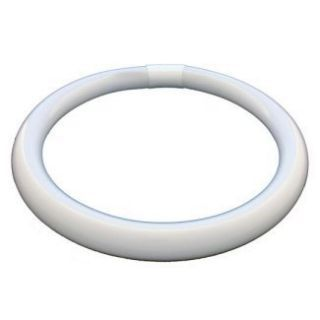
\includegraphics[width=.35\textwidth]{CIRCULAR_TUBE.jpg}
\caption{A circular bar.}
\end{figure}
In this case, we may still model using the heat equation 
\[
\pd{u(x,t)}{t}{} - \kappa\pd{u(x,t)}{x}{2} = f(x,t), \quad 0 < x < 1
\]
with \emph{periodic} boundary conditions
\[
u(1,t) = u(0,t)
\]
and
\[
\pd{u(1,t)}{x}{} = \pd{u(0,t)}{x}{}
\]
for all $t \geq  0$. 
\begin{enumerate}
\item Suppose we are given points on a line 
\[
0 = x_0, \quad x_1, \quad x_2, \quad\ldots,\quad x_N, \quad x_{N+1} = 1.
\]
Construct the finite difference equations for the steady state heat equation 
\[
\kappa\pd{u(x,t)}{x}{2} = f(x), \quad 0 < x < 1
\]
with periodic boundary conditions
\[
u(1) = u(0), \qquad \pd{u(1)}{x}{} = \pd{u(0)}{x}{}.
\]
(You will need to approximate $\pd{u(1)}{x}{}$ and $\pd{u(0)}{x}{}$ using finite differences).  

In particular, specify the finite difference equations at the point $x_1$, the point $x_i$ where $ 1< i <N$, and the last point $x_N$, and write out the matrix system that results from the above discretization. 

\item Does the steady state heat equation with periodic boundary conditions yield a unique solution?  Why or why not?  
\end{enumerate}

%%%%%%%%%%%%%%%%%%%%%%%%%%%%%%%%%%%%%%%%%%%%%%%%%%%%%%%%%%%%

\ifthenelse{\boolean{showsols}}{\input bonus_sol}{}